
\documentclass[numbertotal,blue,toc,wide]{bpslides}

\usepackage{blindtext}

\definecolor{green0}{rgb}{0,0.5,0}
\definecolor{red0}{rgb}{0.8,0,0}
\definecolor{blue0}{rgb}{0,0.2,0.8}
\definecolor{black0}{rgb}{0,0,0}
\definecolor{orange0}{rgb}{1,0.25,0}
\definecolor{magenta0}{cmyk}{0,1,0,0}
\definecolor{purple0}{rgb}{0.5,0,1}

%%%%%%%%%%%%%%%%%%%%%%%%

\title{Title of your presentation}

\subtitle{Subtitle of the presentation}

\author{Author 1\inst{1} \and Author 2\inst{2} \and Author 3\inst{3}}

\institute{\inst{1} Institution 1, \  \inst{2} Institution 2, \  \inst{3} Institution 3}

\conference{Conference/university hosting the talk}

\date{\today}

\leftfoot{Whatever you want to write}

%%%%%%%%%%%%%%%%%%%%%%%%

\begin{document}

\begin{frame}[plain]
	\titlepage
\end{frame}

\begin{frame}{Main options - Colors}\label{firstslide}
\begin{itemize}
\item \texttt{green}: {\color{green0}Lorem ipsum dolor sit amet, consectetur adipiscing elit}.\hfill \note{(default)}
\item \texttt{red}: {\color{red0}Lorem ipsum dolor sit amet, consectetur adipiscing elit}.
\item \texttt{blue}: {\color{blue0}Lorem ipsum dolor sit amet, consectetur adipiscing elit}.
\item \texttt{orange}: {\color{orange0}Lorem ipsum dolor sit amet, consectetur adipiscing elit}.
\item \texttt{black}: {\color{black}Lorem ipsum dolor sit amet, consectetur adipiscing elit}.
\item \texttt{magenta}: {\color{magenta0}Lorem ipsum dolor sit amet, consectetur adipiscing elit}.
\item \texttt{purple}: {\color{purple0}Lorem ipsum dolor sit amet, consectetur adipiscing elit}.
\end{itemize}
\end{frame}

\begin{frame}{Main options - Font typefaces}\label{firstslide}
\begin{itemize}
\item \texttt{helvetica}
\item \texttt{sans}
\item \texttt{iowa}
\item \texttt{palatino}
\item \texttt{bookman}
\item \texttt{termes}
\item \texttt{adventor}
\end{itemize}
\end{frame}

\begin{frame}{Main options - Other options}\label{firstslide}
\begin{itemize}
\item \texttt{hdrule}: add a line below frame title
\item \texttt{numbering}: include slide numbers in the (right) footer
\item \texttt{numbertotal}: include slide number and total number of slides in the (right) footer
\item \texttt{toc}: include a table of contents at the beginning of each section
\begin{itemize}
\item If this option is not selected but the user defines sections in the document, headings will show up in a separate slide at the beginning of each section
\end{itemize}
\item \texttt{wide}: change the aspect ratio of the slides from 4:3 (default) to 16:9
\end{itemize}
\end{frame}

\section{Itemize and enumerate environments}

\subsection{Itemize environment}

\begin{frame}{Itemize}\label{firstslide}
Lorem ipsum dolor sit amet, consectetur adipiscing elit, sed do eiusmod tempor incididunt ut labore et dolore magna aliqua. 
\begin{itemize}
\item Lorem ipsum dolor sit amet, consectetur adipiscing elit, sed do eiusmod tempor incididunt ut labore et dolore magna aliqua.
\item Lorem ipsum dolor sit amet, consectetur adipiscing elit, sed do eiusmod tempor incididunt ut labore et dolore magna aliqua.
\begin{itemize}
\item Lorem ipsum dolor sit amet, consectetur adipiscing elit, sed do eiusmod tempor incididunt ut labore et dolore magna aliqua.
\end{itemize}
\item Lorem ipsum dolor sit amet, consectetur adipiscing elit, sed do eiusmod tempor incididunt ut labore et dolore magna aliqua.
\end{itemize}
\end{frame}

\begin{frame}{Enumerate}{This is how a frame's subtitle looks like}
Lorem ipsum dolor sit amet, consectetur adipiscing elit, sed do eiusmod tempor incididunt ut labore et dolore magna aliqua. 
\begin{enumerate}
\item Lorem ipsum dolor sit amet, consectetur adipiscing elit, sed do eiusmod tempor incididunt ut labore et dolore magna aliqua.
\item Lorem ipsum dolor sit amet, consectetur adipiscing elit, sed do eiusmod tempor incididunt ut labore et dolore magna aliqua. 
\begin{enumerate}
\item Lorem ipsum dolor sit amet, consectetur adipiscing elit, sed do eiusmod tempor incididunt ut labore et dolore magna aliqua. 
\end{enumerate}
\item Lorem ipsum dolor sit amet, consectetur adipiscing elit, sed do eiusmod tempor incididunt ut labore et dolore magna aliqua. 
\end{enumerate}
\end{frame}

\section{Blocks and buttons}

\begin{frame}{Blocks}
\begin{block}{Example of a block}
Lorem ipsum dolor sit amet, consectetur adipiscing elit, sed do eiusmod tempor incididunt ut labore et dolore magna aliqua. Ut enim ad minim veniam, quis nostrud exercitation ullamco laboris nisi ut aliquip ex ea commodo consequat. Duis aute irure dolor in reprehenderit in voluptate velit esse cillum dolore eu fugiat nulla pariatur.
\end{block}
\begin{itemize}
\item Lorem ipsum dolor sit amet, consectetur adipiscing elit, sed do eiusmod tempor incididunt ut labore et dolore magna aliqua.
\item Lorem ipsum dolor sit amet, consectetur adipiscing elit, sed do eiusmod tempor incididunt ut labore et dolore magna aliqua.
\end{itemize}
\end{frame}

\begin{frame}{Buttons}
\vfill
\begin{itemize}
\item Lorem ipsum dolor sit amet, consectetur adipiscing elit, sed do eiusmod tempor incididunt ut labore et dolore magna aliqua.
\item Lorem ipsum dolor sit amet, consectetur adipiscing elit, sed do eiusmod tempor incididunt ut labore et dolore magna aliqua.
\item Lorem ipsum dolor sit amet, consectetur adipiscing elit, sed do eiusmod tempor incididunt ut labore et dolore magna aliqua.
\item Lorem ipsum dolor sit amet, consectetur adipiscing elit, sed do eiusmod tempor incididunt ut labore et dolore magna aliqua.
\end{itemize}
\vfill
\hfill An example of button $\to$ \button{firstslide}{back to first slide}
\end{frame}

\section{Tables and figures}

\begin{frame}{Tables}
\begin{table}
\centering
\caption{Heading of the table}
\begin{tabular}{cccc} \toprule
 & Mean & Median & Std Desvi.\\ \midrule
Variable 1 & $1150$ & 900 & 235 \\ 
Variable 2 & $430$ & 300 & 57 \\ 
Variable 3 & $367$ & 210 & 113 \\ \bottomrule
\end{tabular}
\end{table}
\end{frame}

\begin{frame}{Figures}
\begin{figure}
\centering
\caption{Heading of the figure}
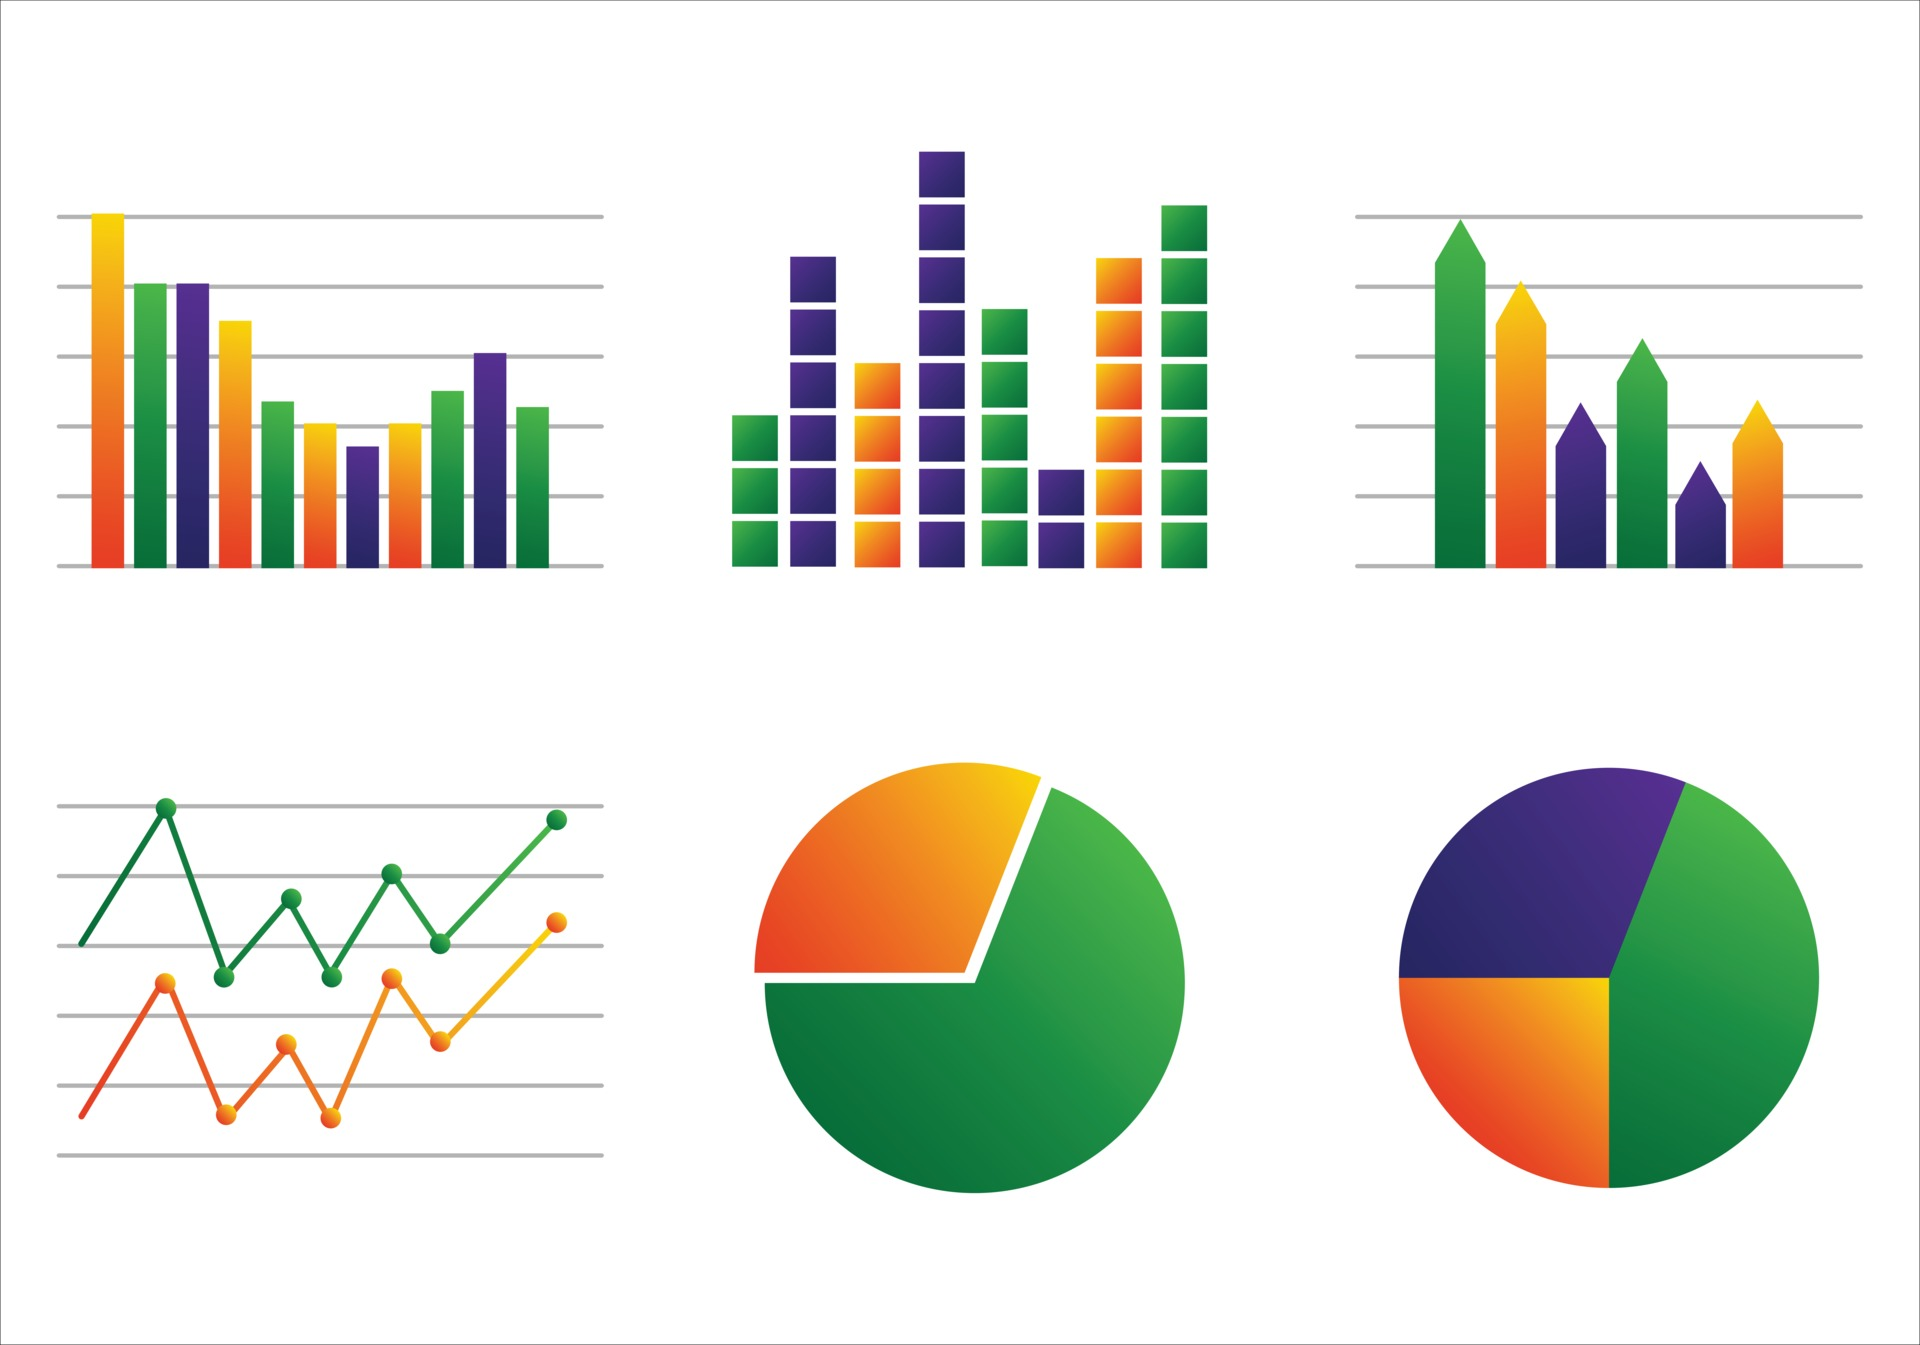
\includegraphics[width=0.9\paperheight]{graph}
\end{figure}
\end{frame}

\section{New commands}

\begin{frame}{New commands}
	\begin{itemize}
	\item \texttt{$\backslash$leftfoot$\{$whatever$\}$} displays ``whatever'' in the bottom-left corner
	\item \texttt{$\backslash$conference$\{$the place$\}$} displays the place hosting the talk in the title page
	\item \texttt{$\backslash$paper$\{$Author$\}\{$Year$\}$} displays \paper{Author}{Year}
	\item \texttt{$\backslash$paperalt$\{$Author$\}\{$Year$\}$} displays \paperalt{Author}{Year}
	\item \texttt{$\backslash$note$\{$some text$\}$} displays \note{some text}
	\item \texttt{$\backslash$under$\{$some other text$\}$} displays \under{some other text}
	\item \texttt{$\backslash$vs}: equivalent to \texttt{$\backslash$vspace$\{$0.1cm$\}$}
	\item \texttt{$\backslash$hs}: equivalent to \texttt{$\backslash$hspace$\{$0.1cm$\}$}
	\end{itemize}
\end{frame}

\end{document}
